\section{Introduction} % (fold)
\label{sec:introduction}
Computers around the world run at notoriously low utilization levels. Previous work~\cite{Kurt:07,Judy:04} has estimated that most of the desktop PCs remain powered up outside of normal work hours and only 4\% of them go to sleep when idle. The home desktop is typically on for one third of the day and is being used only half the time. Data centers also face the same problem of low utilization, as low as 10-50\%~\cite{Luiz:07,Albert:09}. This combined with the lack of energy proportional computers (as seen in Figure~\ref{fig:active-idle-power}) mean that a bulk of the energy used by computing (and ancillary services indirectly) is spent not on cycles of useful work, but on cycles waiting for work to be scheduled. Figure~\ref{fig:r-utilization} shows the utilization\footnote{The data is from the month of Nov '09. If at all the utilization would be abnormally high given that it is the final month of lectures.} of the ``R-Cluster'' in Soda Hall across a one month period. It can be clearly seen that the utilization in the R-cluster very rarely increases beyond 15\%. Bruce Nordman~\cite{Bruce:08} estimates that the total power used by networked devices in the US alone is as much as 150TWh. The Treehugger blog~\cite{TreeHugger:08} estimates that there are 30.3 million servers around the world and they run at an average utilization rate of 15\%. Even at 30\% utilization and assuming that the servers run at 100W at idle and 150W at peak utilization~\cite{Yuvraj:09}, this is the equivalent of a {\em 3484.5MW} light bulb. This translates into a yearly power bill of 1244 billion USD of which 763 billion USD was wasted without doing useful work. To put this in perspective, "computing servers use one-tenth of all the energy generated by nuclear reactors.~\cite{Robert:06}. 

\begin{figure}[ht]
\centering
\begin{center}
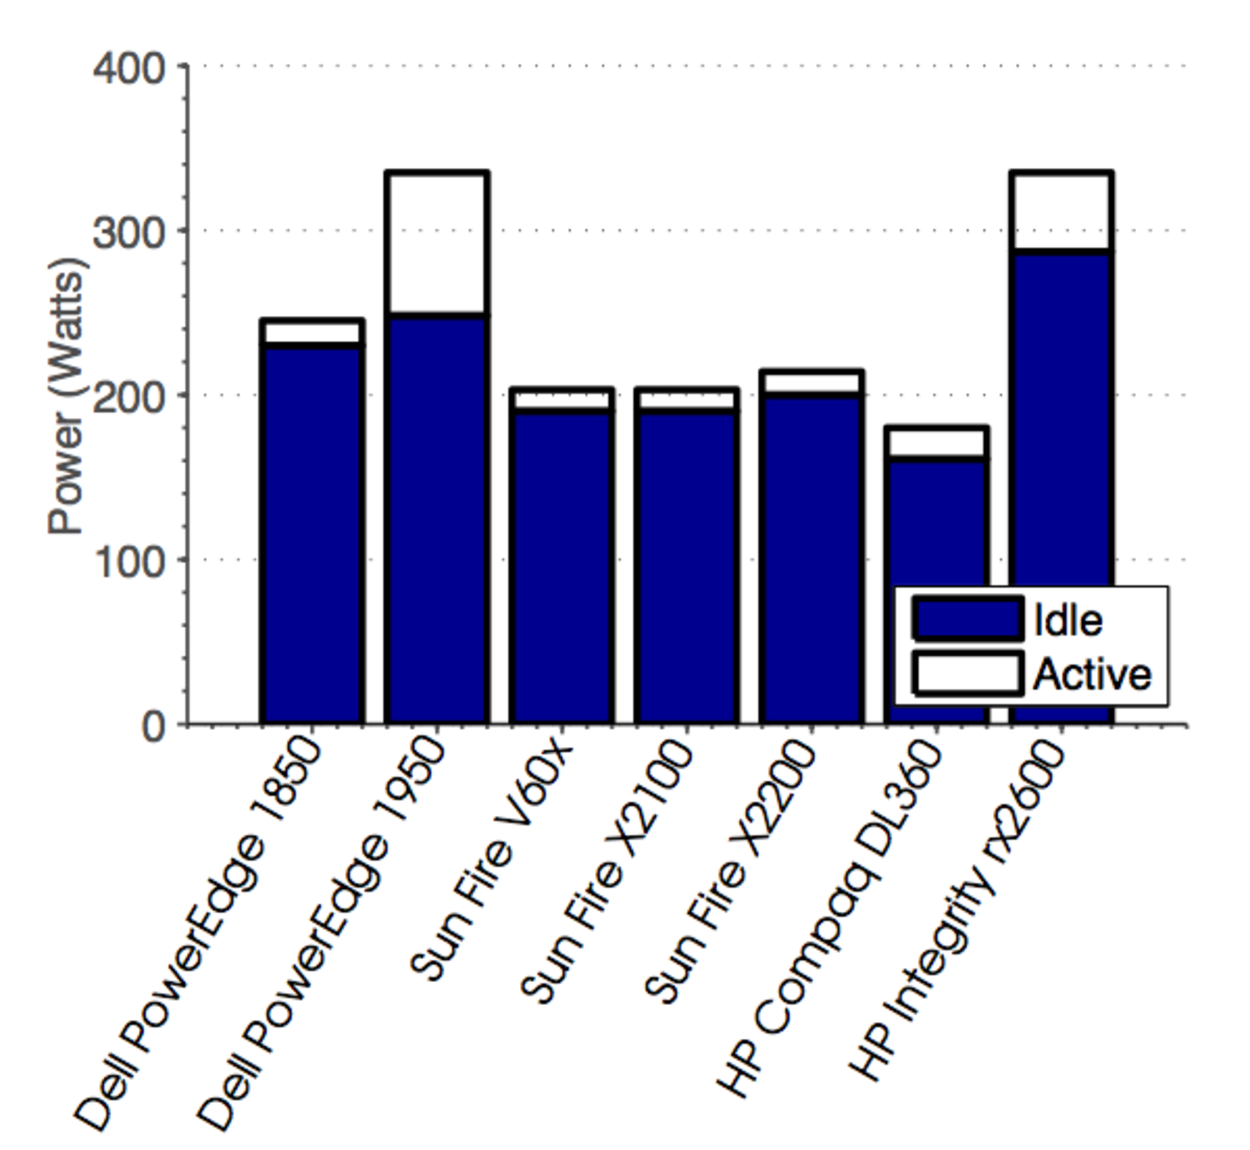
\includegraphics[width=3.0in]{graphs/steve-TR-idle-active.pdf}
\vspace{-0.1in}
\caption{{\normalsize Comparison of power usage of various nodes in active and idle states (Figure from~\cite{Dawson-Haggerty:09})}\label{fig:active-idle-power}}
\vspace{-0.1in}
\end{center}
\end{figure}

\begin{figure}[ht]
\centering
\begin{center}
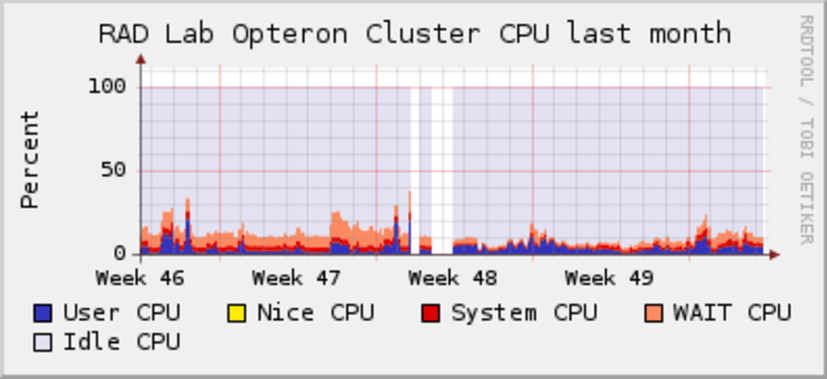
\includegraphics[width=3.0in]{graphs/Rcluster-nov-usage.pdf}
\vspace{-0.1in}
\caption{{\normalsize R-Cluster utilization over a month}\label{fig:r-utilization}}
\vspace{-0.1in}
\end{center}
\end{figure}

Energy consumption in computing devices has attracted much attention in the past few years. This has been in part due to the rise of centralized computing infrastructures in the form of data centers. PUE (Power Usage Efficiency) is a metric that is often used to compare the efficiency of a data center. PUE is defined to be:
\begin{scriptsize}
    \begin{equation}
        PUE = \frac{Total~energy~used~in~facility}{Energy~consumed~by~computing~infrastructure}
        \label{eq:pue}
    \end{equation}
\end{scriptsize}
Historically much work has focused on improving this specific metric by introducing innovative data center design; getting cooling for free with outside air~\cite{Neil:06}, operating at higher temperatures~\cite{Ratnesh:05}, reducing power supply loss by using smaller UPSs, etc. However, with today's data centers attaining PUEs as low as 1.035~\cite{Sandia:09} (i.e., 3.5W spent elsewhere for every 100W spent on computing), focus has moved back to reducing the power used by compute servers. Reducing the power consumption of computing nodes also reduces total cost of ownership indirectly~\cite{Luiz:07} by requiring lesser power for cooling as the heat dissipated by CPUs reduces.

However, PUE as a metric itself is flawed in the sense that while it is representative of datacenter operations, it is not representative of the work done per watt of energy\footnote{This is an idea of a metric floated by Prof. David Culler}. A typical metric should calculate the energy used per instruction of useful work. This can be approximated to CUE (Computation Usage Efficiency):
\begin{scriptsize}
    \begin{equation}
        CUE = \frac{Total~energy~used~in~facility}{Energy~consumed~by~computers~doing-work}
        \label{eq:cue}
    \end{equation}
\end{scriptsize}

Section~\ref{sec:related_work} describes other literature also attempting to reduce power usage on computing nodes and create a more power proportional computer. We describe the architecture of our ``Clean Clusters'' software suite and its dependent software in Section~\ref{sec:architecture}. We then analyze the overhead of ``race to sleep'' on a real cluster and apply our learning on a set of HPC workload traces in Section~\ref{sec:results}. A description of the simulator we built to analyze performance and energy benefits is described in detail in Section~\ref{sub:trace_driven_simulation}.

% Data from http://www.eecs.berkeley.edu/Pubs/TechRpts/2009/EECS-2009-140.html
% More data 

% section introduction (end)

